%%%%%%%%%%%%%%%%%%%%%%%%%%%%%%%%%%%%%%%%%%%
%%% DOCUMENT PREAMBLE %%%
\documentclass[12pt]{report}
\usepackage[english]{babel}
%\usepackage{natbib}
\usepackage{url}
\usepackage[utf8x]{vietnam}
\usepackage{amsmath}
\usepackage{graphicx}
\graphicspath{{images/}}
\usepackage{parskip}
\usepackage{fancyhdr}
\usepackage{vmargin}
\setmarginsrb{3 cm}{2.5 cm}{3 cm}{2.5 cm}{1 cm}{1.5 cm}{1 cm}{1.5 cm}

\usepackage{tabularx}

\title{Assignment 2}								
% Title
\author{}						
% Author
\date{March 2019}
% Date

\makeatletter
\let\thetitle\@title
\let\theauthor\@author
\let\thedate\@date
\makeatother

\pagestyle{fancy}
\fancyhf{}
\rhead{\theauthor}
\lhead{\thetitle}
\cfoot{\thepage}
%%%%%%%%%%%%%%%%%%%%%%%%%%%%%%%%%%%%%%%%%%%%
\begin{document}

%%%%%%%%%%%%%%%%%%%%%%%%%%%%%%%%%%%%%%%%%%%%%%%%%%%%%%%%%%%%%%%%%%%%%%%%%%%%%%%%%%%%%%%%%

\begin{titlepage}
	\centering
    \vspace*{0.5 cm}
   % \includegraphics[scale = 0.075]{bsulogo.png}\\[1.0 cm]	% University Logo
\begin{center}
    \textsc{\Large   Ho Chi Minh City University of Technology
	}\\[0.3 cm]
	
\includegraphics[scale=0.4]{hcmut.png} \\
	$\ast\ast\ast$
	\\[3.0cm]
\end{center}% University Name
	\textsc{\LARGE COMPUTER NETWORK}\\[0.5 cm]				% Course Code
	\rule{\linewidth}{0.2 mm} \\[0.4 cm]
	{ \huge \bfseries \thetitle}\\
	\rule{\linewidth}{0.2 mm} \\[1.5 cm]
	
	\begin{minipage}{0.0\textwidth}
		\begin{flushleft} \large
		%	\emph{Submitted To:}\\
		%	Name\\
          % Affiliation\\
           %contact info\\
			\end{flushleft}
			\end{minipage}~
			\begin{minipage}{0.5\textwidth}
            
			\begin{flushleft} \large
			GVHD: BÙI XUÂN GIANG \\
			\rule{\linewidth}{0.2 mm}
			Thành viên: \\
			1. ĐINH QUỐC CƯỜNG - 1710712\\
			2. ĐINH HOÀNG KIM - 1711872\\
			3. NGUYỄN THÀNH KHÁNH AN - 1710433
		\end{flushleft}
           
	\end{minipage}\\[2 cm]
	 
    
    
	
\end{titlepage}

%%%%%%%%%%%%%%%%%%%%%%%%%%%%%%%%%%%%%%%%%%%%%%%%%%%%%%%%%%%%%%%%%%%%%%%%%%%%%%%%%%%%%%%%%

\tableofcontents
\pagebreak

%%%%%%%%%%%%%%%%%%%%%%%%%%%%%%%%%%%%%%%%%%%%%%%%%%%%%%%%%%%%%%%%%%%%%%%%%%%%%%%%%%%%%%%%%
\renewcommand{\thesection}{\arabic{section}}

\section{Giới thiệu đề tài}

	Nhằm xây dựng một trường đại học hiện đại, thân thiện và sử dụng năng lượng
tiết kiệm. Trường đại học Bách Khoa đang giao cho Khoa Khoa học và Kỹ thuật Máy
Tính nhiệm vụ nghiên cứu và triển khai lắp đặt hệ thống giám sát các hoạt động của
sinh viên tại các tòa nhà và các thiết bị đo nhiệt độ, độ ẩm, ánh sáng trong các phòng
học nhằm giảm chi phí về năng lượng. \\\\
	Hệ thống được triển khai thí điểm ở các tòa
nhà H6 tại cơ sở 2. Để phục vụ tốt cho hoạt động của hệ thống, Khoa cần thiết kế
mới và triển khai hệ thống mạng ở tòa nhà này. Các nhóm sinh viên đang học môn
Mạng máy tính được mờ tham gia tư vấn và đưa ra giải pháp pháp với yêu cầu của
tòa nhà hiện tại.

\section{Phân tích hệ thống}
	\subsection{Mục đích}
		\begin{itemize}
			\item Xây dựng hệ thống giám sát các hoạt động của sinh viên tại các tòa nhà và các thiết bị IoT như các cảm biến ánh sáng, nhiệt độ, các camera giám sát,...
			\item Mục tiêu: Giảm chi phí về năng lượng của tòa nhà.
		\end{itemize}
	\subsection{Phạm vi áp dụng}
		Hệ thống được triển khai thí điểm ở tòa H6 - Đại học Bách Khoa cơ sở 2. Tòa nhà gồm có 7 tầng:
		\begin{itemize}
			\item Tầng 1:
			\begin{itemize}
				\item 7 phòng học lớn.
				\item 6 phòng học nhỏ.
				\item 1 phòng server.
			\end{itemize}
			\item Tầng 2, 3, 4, 5:
			\begin{itemize}
				\item 7 phòng học lớn.
				\item 7 phòng học nhỏ.
			\end{itemize}
			\item Tầng 6, 7, 8:
			\begin{itemize}
				\item 4 phòng học nhỏ.
				\item 7 phòng thực hành.
			\end{itemize}
		Ngoài ra ở tầng 7 còn đặt 1 phòng hành chính.
		\end{itemize}
	
	\subsection{Yêu cầu}
		Các phòng sẽ được trang bị các thiết bị IoT gồm có các cảm biến nhiệt độ, ánh sáng, điều khiển đèn, điều khiến máy lạnh... Ngoài hành lang được lắp thêm các camera giám sát, chi tiết được mô tả như sau:
		\begin{itemize}
			\item Các phòng học lớn sẽ được trang bị 6 cảm biến nhiệt độ, 6 cảm biến ánh sáng, một máy tính, một thiết bị điều khiển đèn.
			\item Các phòng học nhỏ sẽ được trang bị 3 cảm biến nhiệt độ, 3 cảm biến ánh sáng, 1 máy tính và 1 thiết bị điều khiển đèn.
			\item Các phòng thực hành được trang bị 6 cảm biến nhiệt độ, 6 cảm biến ánh sáng, 1 thiết bị điều khiển đèn, 1 thiết bị điều khiển máy lạnh, 12 máy tính thực hành + 1 máy tính giảng viên. Các máy tính này sẽ download khoảng 200MB một ngày và gửi khoảng 10 email, mỗi email có dung lượng tối đa 10MB.
			\item Dữ liệu từ các cảm biến sẽ có kích thước 32Kb và được đo 1 phút một lần và gửi về Server với chu kỳ 5 phút 1 lần.
			\item Dữ liệu từ các camera sẽ được lưu trực tiếp lên Server 24/24.	
		\end{itemize}
	
\newpage
\section{Bản thiết kế vật lý}
	
	\subsection{Các thiết bị sử dụng}
		\begin{center}
			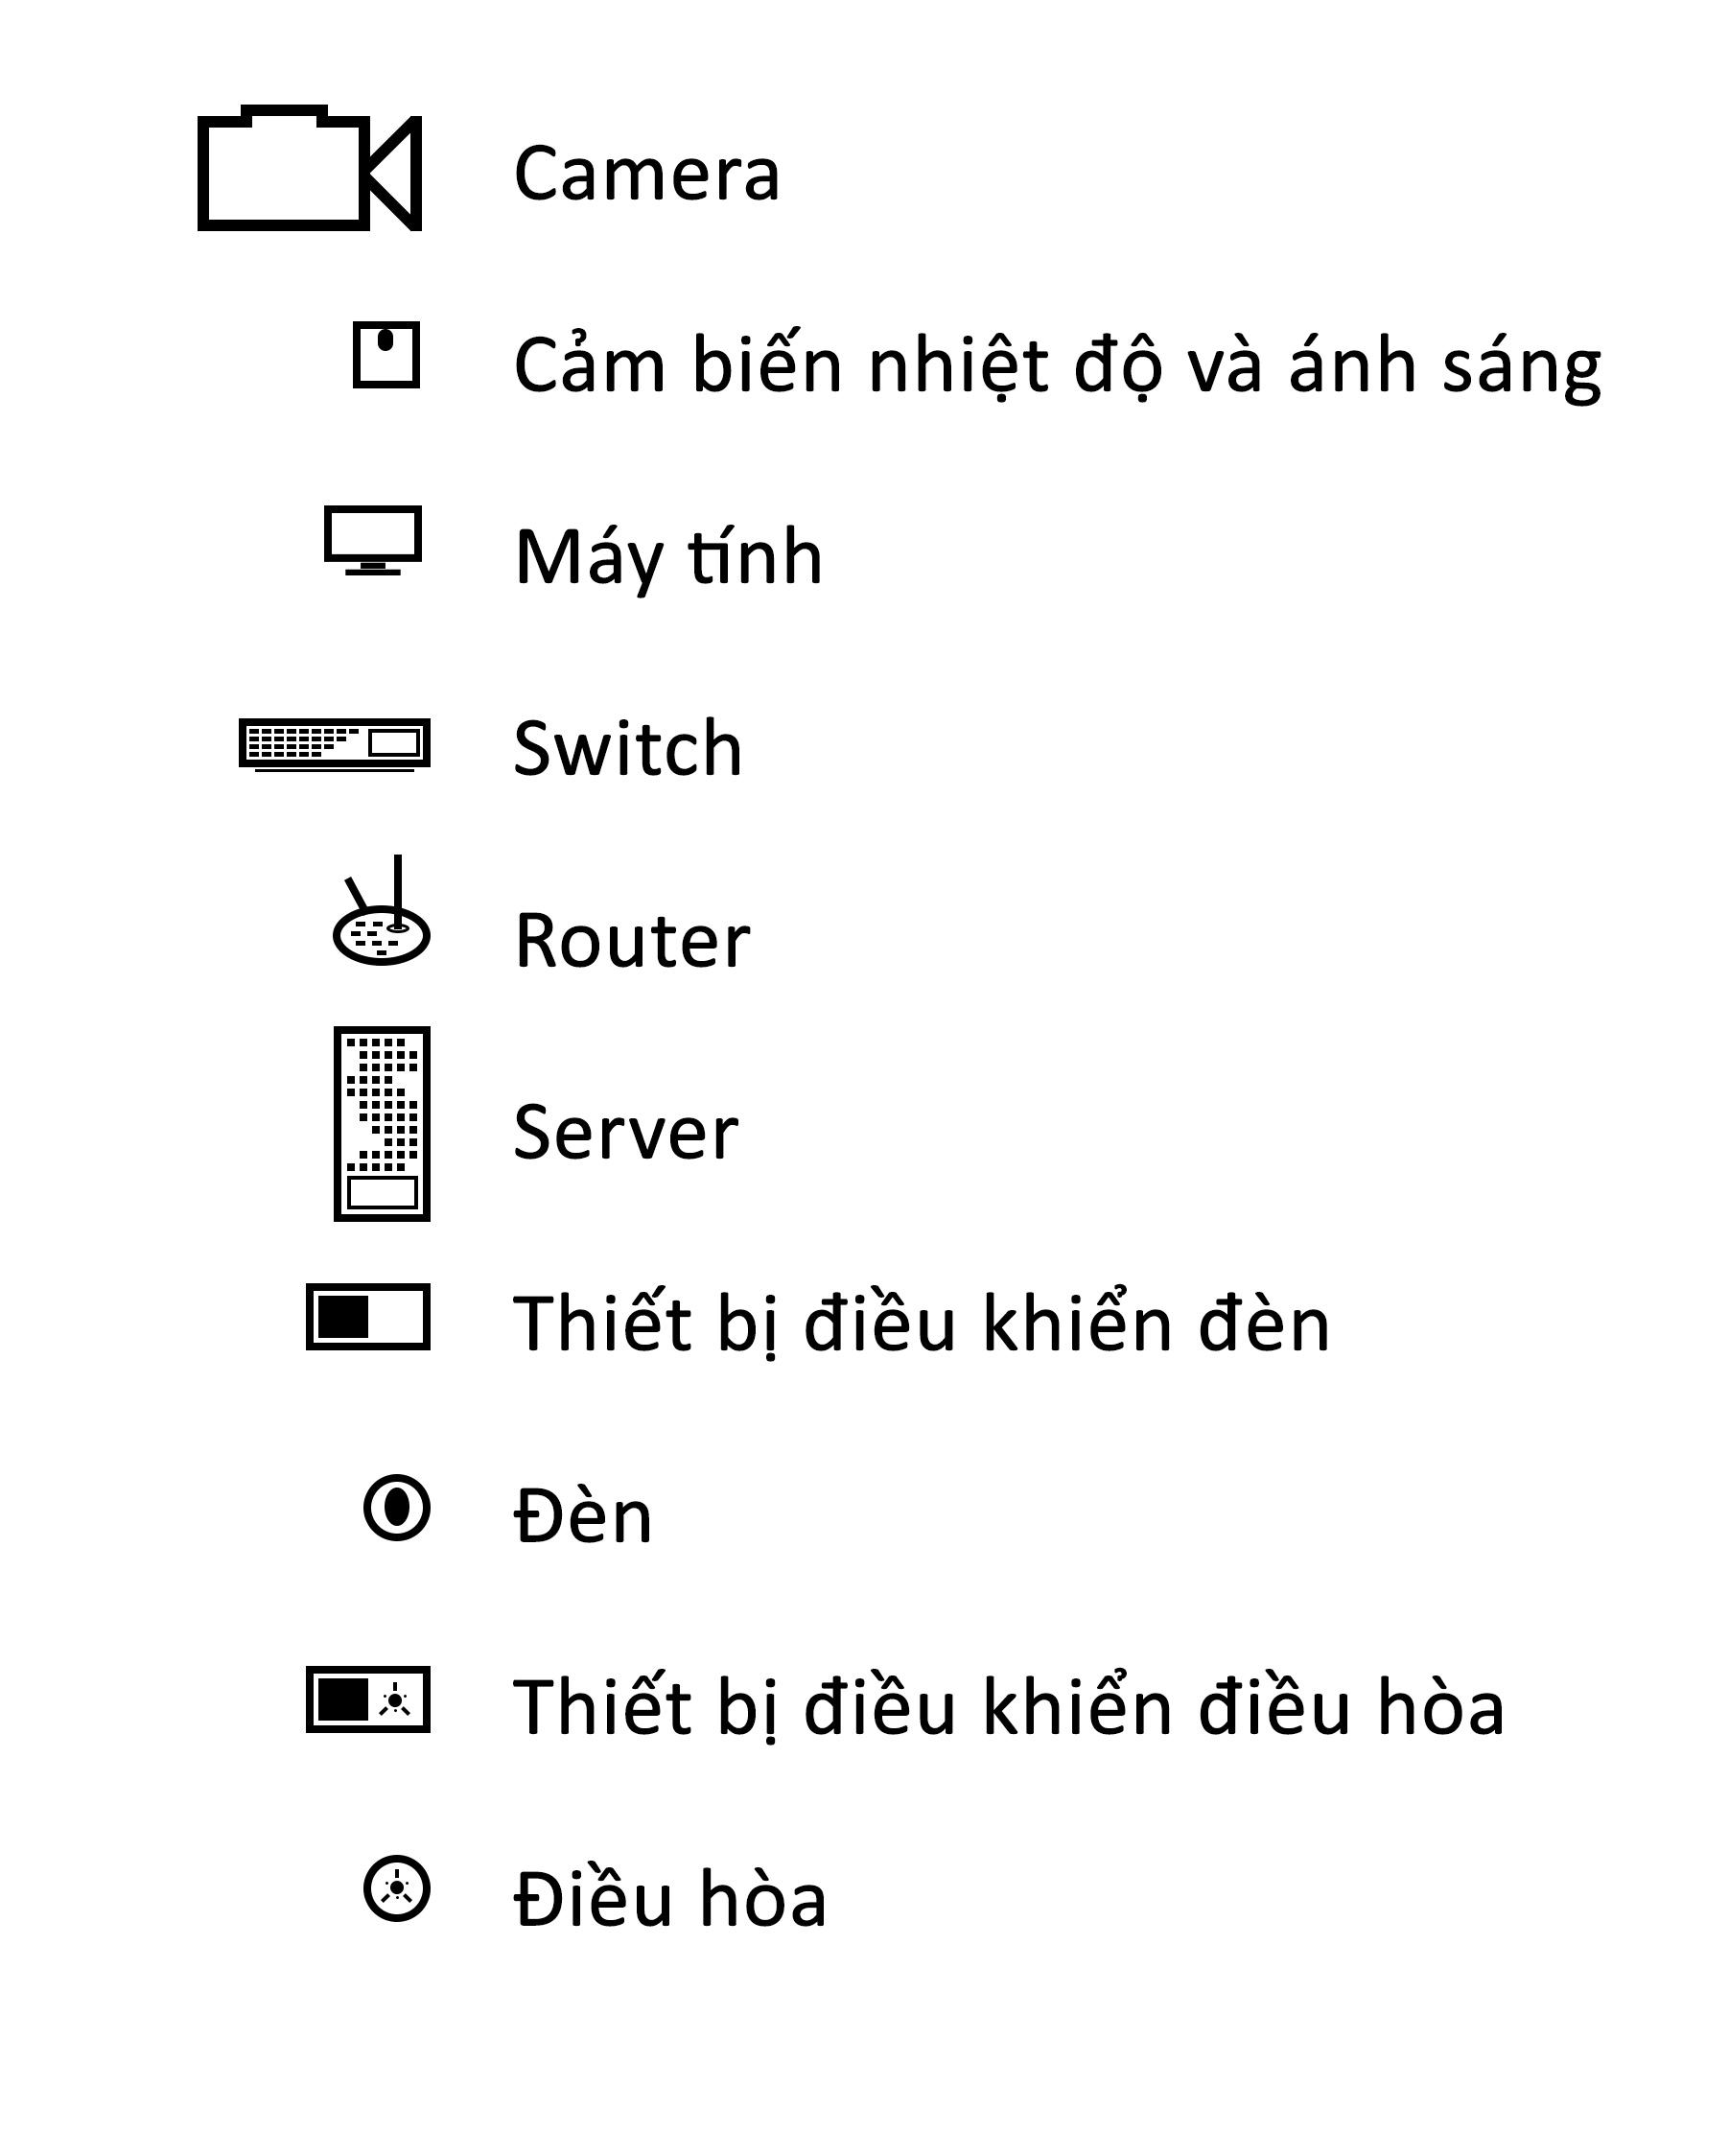
\includegraphics[scale=0.15]{device.jpg} \\
		\end{center}
	
	\newpage
	\subsection{Các loại phòng}

		\subsubsection{Phòng học lớn}
		
			\begin{itemize}
				\item 6 cảm biến ánh sáng
				\item 6 cảm biến nhiệt độ
				\item 1 thiết bị điều khiển đèn
				\item 1 máy tính
				\item 1 switch
			\end{itemize}
		
			\begin{center}
				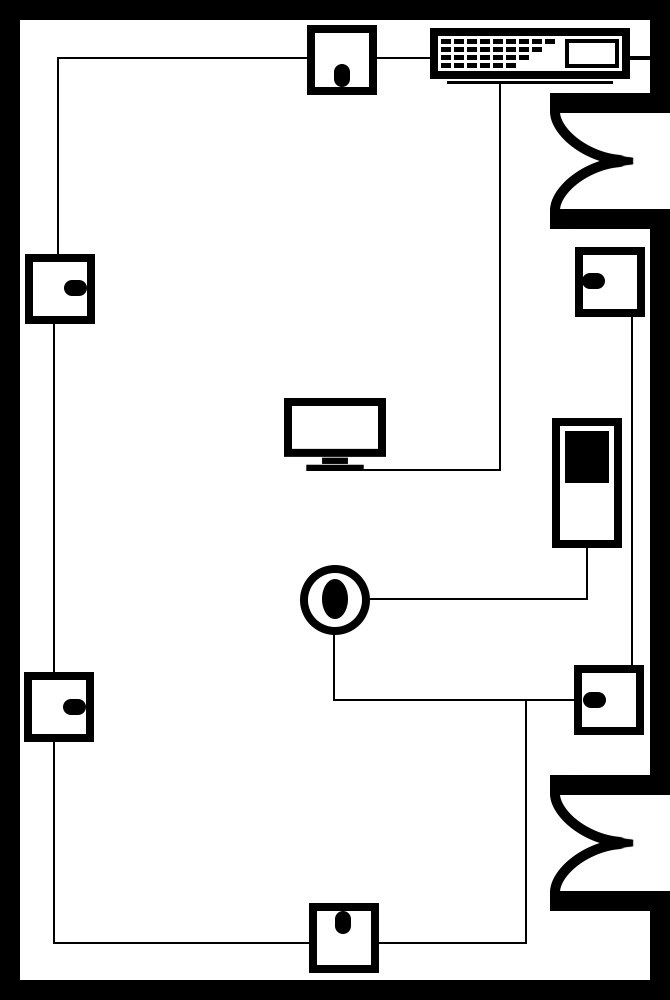
\includegraphics[scale=0.3]{roomBig.jpg} \\
			\end{center}
		
		\newpage
		\subsubsection{Phòng học nhỏ}
		
			\begin{itemize}
				\item 3 cảm biến ánh sáng
				\item 3 cảm biến nhiệt độ
				\item 1 thiết bị điều khiển đèn
				\item 1 máy tính
				\item 1 switch
			\end{itemize}
		
			\begin{center}
				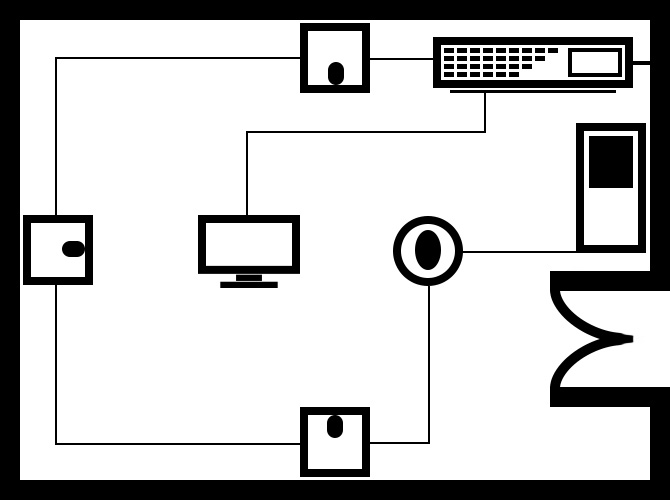
\includegraphics[scale=0.3]{roomSmall.jpg} \\
			\end{center}
		
		\newpage
		\subsubsection{Phòng đặt Server}
		
			\begin{itemize}
				\item 3 cảm biến ánh sáng
				\item 3 cảm biến nhiệt độ
				\item 1 thiết bị điều khiển đèn
				\item 1 thiết bị điều khiển điều hòa
				\item 1 router
				\item 1 switch
				\item 1 server
				\item 1 máy tính
			\end{itemize}
			
			\begin{center}
				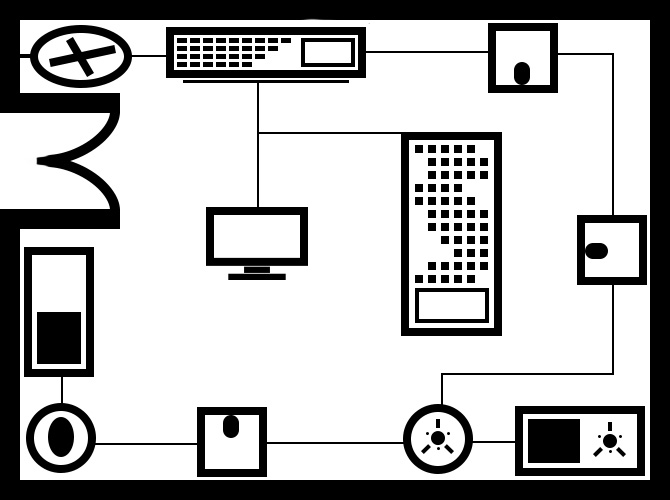
\includegraphics[scale=0.3]{roomServer.jpg} \\
			\end{center}
		
		\newpage
		\subsubsection{Phòng học thực hành}

			\begin{itemize}
				\item 6 cảm biến ánh sáng
				\item 6 cảm biến nhiệt độ
				\item 1 thiết bị điều khiển đèn
				\item 1 thiết bị điều khiển điều hòa
				\item 1 switch
				\item 13 máy tính
			\end{itemize}
			
			\begin{center}
				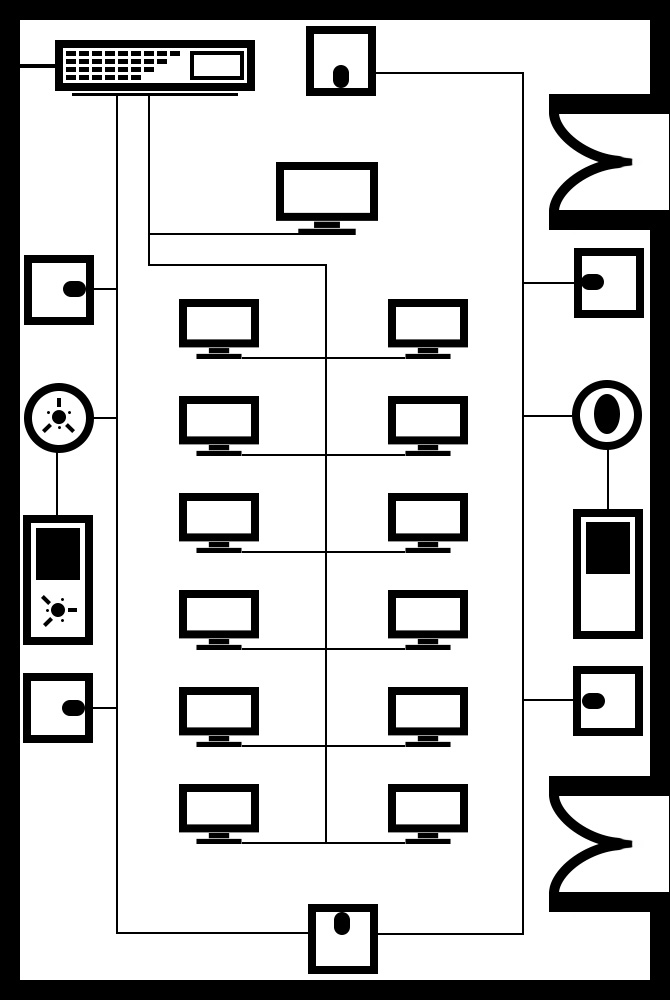
\includegraphics[scale=0.3]{roomLab.jpg} \\
			\end{center}

		\newpage
		\subsubsection{Phòng hành chính}
		
			\begin{itemize}
				\item 6 cảm biến ánh sáng
				\item 6 cảm biến nhiệt độ
				\item 1 thiết bị điều khiển đèn
				\item 1 thiết bị điều khiển điều hòa
				\item 1 switch
				\item 10 máy tính
			\end{itemize}
		
			\begin{center}
				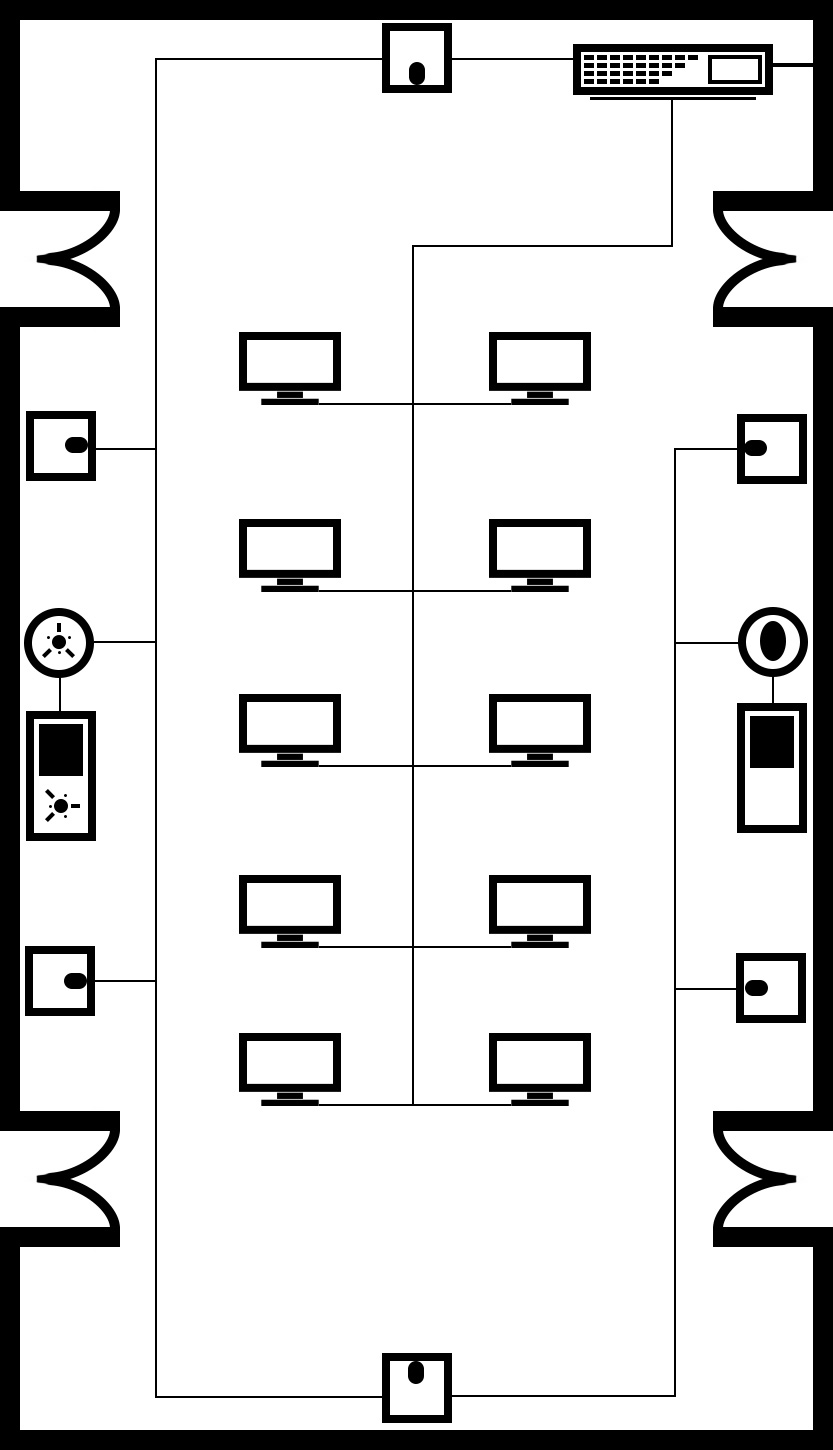
\includegraphics[scale=0.25]{roomMain.jpg} \\
			\end{center}
	
	\newpage
	\subsection{Tầng 1 - đặt phòng Server}
		
		\begin{center}
			\includegraphics[scale=0.09]{h6-f1.png} \\
		\end{center}
		
		\newpage
		\begin{itemize}
			\item Switch tổng
			\begin{itemize}
				\item Router tầng 1 -> Switch tầng 1
				\begin{itemize}
					\item Switch
					\begin{itemize}
						\item 4 camera giám sát
					\end{itemize}
					\item Wireless WiFi
					\item Các switch của mỗi phòng
				\end{itemize}					
			\end{itemize}
			
		\end{itemize}
	
	\newpage
	\subsection{Tầng 7 - đặt phòng hành chính}

		\begin{center}
			\includegraphics[scale=0.09]{h6-f7.png} \\
		\end{center}
		
		\newpage
		\begin{itemize}
			\item Dẫn từ Switch tổng
			\begin{itemize}
				\item Router tầng 7 -> Switch tầng 7
				\begin{itemize}
					\item Switch
					\begin{itemize}
						\item 4 camera giám sát
					\end{itemize}
					\item Wireless WiFi
					\item Các switch của mỗi phòng
				\end{itemize}					
			\end{itemize}
			
		\end{itemize}




\section{Tính toán dung lượng lưu trữ, đường truyền}



\section{Sơ đồ luận lý}

\section{Kĩ Thuật sử dụng}
	\subsection{Chia VLAN}
	Các tầng được cấu hình VLAN riêng:
	\begin{table}[!h]
		\centering
		\begin{tabularx}{0.8\textwidth} { | >{\centering\arraybackslash}X | >{\centering\arraybackslash}X |}
			\hline
			Name & VLAN Number \\ \hline
			Lau1  & 10  \\ 		\hline
			Lau2  & 20  \\ 		\hline
			Lau3  & 30  \\ 		\hline
			Lau4  & 40  \\ 		\hline
			Lau5  & 50  \\ 		\hline
			Lau6  & 60  \\ 		\hline
			Lau7  & 70  \\ 		\hline
			Lau8  & 80  \\ 		\hline
			
		\end{tabularx} 
		\caption{Bảng chia VLAN}

	\end{table}
	\subsection{Subinterface}
	\subsection{Định tuyến tĩnh}
	\subsection{Cấp IP Động}

\section{Danh mục thiết bị và ước lượng kinh phí}

\section{Đánh giá}

\end{document}